%
% File acl2017.tex
%
%% Based on the style files for ACL-2015, with some improvements
%%  taken from the NAACL-2016 style
%% Based on the style files for ACL-2014, which were, in turn,
%% based on ACL-2013, ACL-2012, ACL-2011, ACL-2010, ACL-IJCNLP-2009,
%% EACL-2009, IJCNLP-2008...
%% Based on the style files for EACL 2006 by 
%%e.agirre@ehu.es or Sergi.Balari@uab.es
%% and that of ACL 08 by Joakim Nivre and Noah Smith

\documentclass[11pt,a4paper]{article}
\usepackage[hyperref]{acl2017}
\usepackage{times}
\usepackage{latexsym}
\usepackage{xcolor}

\usepackage{url}

\aclfinalcopy % Uncomment this line for the final submission
%\def\aclpaperid{***} %  Enter the acl Paper ID here

%\setlength\titlebox{5cm}
% You can expand the titlebox if you need extra space
% to show all the authors. Please do not make the titlebox
% smaller than 5cm (the original size); we will check this
% in the camera-ready version and ask you to change it back.

% added
\usepackage{graphicx}
\usepackage{amsmath}
\usepackage{dsfont} %to have \mathds{1}

\newcommand\BibTeX{B{\sc ib}\TeX}

\title{Identification and quantification of colours in children's drawings}

\author{Christelle Cocco ${}^1$, Rapha\"el Cer\'e ${}^2$, Aris Xanthos, ${}^3$  Pierre-Yves Brandt ${}^1$\\
  ${}^1$Institute for Social Sciences of Religions / University of Lausanne, Switzerland \\
  ${}^2$Department of Geography and Sustainability / University of Lausanne, Switzerland \\
  ${}^3$Department of Language and Information Sciences / University of Lausanne, Switzerland \\
  {\tt \{Christelle.Cocco, Raphael.Cere, Aris.Xanthos, Pierre-Yves.Brandt\}@unil.ch} \\
%  \And
%  Second Author \\
%  Affiliation / Address line 1 \\
%  Affiliation / Address line 2 \\
%  Affiliation / Address line 3 \\
%  {\tt email@domain} \\
  }


\date{}
\begin{document}
\maketitle
\begin{abstract}
{\color{red}[[TO UPDATE AT THE END]}
{\color{gray}Children's drawings reveal that developing colour retrieval technics
must consider various aspects of what is a colour from the flow of
energy (for physics) to discrete information (for humantities and human
sciences). Hence, the proposed method deals with color variety measures
and colours quantifications upon the drawing to respond at specific
queries e.g. ``Which colours appear?'', or ``How much yellow appears?''.}
\end{abstract}


\section{Introduction}\label{introduction}
\label{sec:introduction}

In computer vision, there are well developed techniques to analyse and retrieve natural images (e.g.~pictures or videos). {\color{red} [Mettre une ref globale -> livre computer vision]}
However, the status of the image in humanities or in human sciences depends more on the perception of the image. Moreover, the images are not necessarily natural (e.g.~paintings or drawings). {\color{red} [Ref sur les peintures]} Therefore, specific techniques need to be developed according to precise research questions of humanities.

For the multicultural and interdisciplinary project: ``Drawings of gods''\footnote{This project is supported by the Swiss National Science Foundation (SNSF), grant number: CR11\textbar1\_156383.}, whose the main fields are developmental psychology and psychology of religion, children's drawings of gods were collected in several countries \cite[for more details about this project, see \textit{e.g.}][]{BrandtKagataSpittelerGillieronPaleologue2009,Dandarova2013,DandarovaRobertDessartSerbaevaEtAl2016}.\footnote{The database of the project is available on \url{http://ddd.unil.ch/}.} 
In order to analyse these drawings, it would be helpful to identify and quantify the colours used by the children in their drawings. 
Indeed, several research questions in the project are related to colours, such as ``Which colours are used to draw god?'', ``Are the same colours utilised in all countries?'', ``Did older children use more or less colours than younger ones?'' {\color{red} ** PYB **, une question a ajouter?}

To answer this type of questions, the main steps are 1) to define a set of colours; 2) to select a colour space; 3) to assign a colour to each pixel; 4) to count the number of colours in each drawing.

Concerning the first step, although it is possible to obtain precise values defining the colour of a pixel with a computer, there is no universal colour set.
It is even difficult to align the perception of two humans (see section~\ref{sec:set_col_definition})
Indeed, the human colour perception occurs through the radiance incident upon
the retina on which three photoreceptor cells, named cones, are located.
Only these three photoreceptors (corresponding to the \emph{Red}, \emph{Green} and \emph{Blue} numerical components (RGB) of a pixel) are necessary to describe a colour using appropriate spectral functions. Standard curves have been adopted in 1931 by the \textit{Commission Internationale de l'Eclairage} (CIE) to specify the colour by those three numbers from spectral power distribution transformation.

Although the CIE standard exists, only computers are able to assign
those three numbers to a colour in a precise manner. Therefore, any
human assignment is basically obsolete due to the influence of an
individual's interpretation of the colour. 
%(e.g. ``Where can I put a threshold between red and orange?'', ``Is it not already brown?'').
Moreover, the human perception of colour distributions of an image can be
drastically different from recorded colour images in terms of vision \cite[see \textit{e.g.}][]{jobson1997} and,
respectively, in terms of perception depending on the context (\textit{e.g.}
\emph{Chubb illusion}  \cite{ChubbSperlingSolomon1989} or \emph{Checker shadow illusion}\footnote{See \textit{e.g.} \url{http://www.michaelbach.de/ot/lum-adelsonCheckShadow/index.html}}) and on the experience of the human visual system \cite[see \textit{e.g.}][]{LottoPurves2001}.


Besides this, this paper focusses on a children's drawing dataset. 
The particularity of this kind of image depends on the drawer's
colour choices. It can be intentional according to his/her own
perception and his/her human singularity or constraints according to
colour availability. Subsequently, the resulting object analysis is
technically constrained: the final colours are altered by the
digitalisation encoding, as well as the quantification of colours.


\section{State of the art}
Most of the researches about colours in computer vision concern the field of image segmentation \cite[see \textit{e.g.}][]{ChengSun2000,ChenPappasMojsilovicEtAl2005,HanmandluVermaSusanEtAl2013} or image retrieval \cite[see \textit{e.g.}][]{DengManjunathKenneyEtAl2001,RaoKumar2015,ZhangZhangYaoEtAl2016}.

For the former (image segmentation), the aim is to segment the image according to the object, often on pictures, and thus to find a set of pixels with quite the same colour. For instance, as proposed by \citet[][p. 445]{GonzalezWoods2008}, the first step is to define an "average" colour of pixels of interest which are part of the image.

The aim of the latter (image retrieval) is to find which images of a dataset correspond to
the one stated as the query, and therefore to determine if the colours of the query and those of the dataset are similar. 
Thus, in both cases, there are no need to determine which colour it is (only which pixels have similar colours), unlike this contribution.


There are also some colour researches in computer vision in the field of object detection or recognition \cite[see \textit{e.g.}]{khan2012}, using sometimes also colour names \cite[see \textit{e.g.}]{khan2013}. 
Nevertheless, their aims differed from the one found in the human sciences and described above. Furthermore, all these methods are developed to treat pictures and not drawings.

However, a number of previous researches in computer vision proposed promising
descriptors such as colour histograms \cite[see \textit{e.g.}][]{sun2006}, colour names
\cite{weijer2009, lindner2013} through mapping learned from images, or parametric models for automatic colour naming (with each colour category modeled as a fuzzy set with a parametric membership function) \cite{benavente2008}.  


When the aim is still to find colour groups, the
K-means algorithm is often used \cite[see e.g.][]{yendrikhovskij2001,konyushkova2015,hulee2007}. However, there are two main
drawbacks with this method: 1) it is necessary to define the number of
clusters (K), thus the number of colours \textit{a priori}; 2) for each cluster,
we can obtain a mean of colours belonging to this cluster and these
means can be difficult to name and to distinguish, or to compare between two images.
More specifically, the paper of \cite{konyushkova2015} proposes a solution closer to the aim of finding
the set of colours displayed in children's drawings of gods.

\citet{kimbaelee2007} proposed a method to detect the colours in drawings highly similar to the one proposed here, the main difference being that they use the Munsell colour system (see section~\ref{sec:colour-space}) and they start with 15 colours instead of 117 (section~\ref{sec:identification}).

To answer questions in humanities and human sciences, it is necessary to develop specific
techniques, since the aim is not to precisely find the nuance/shade of the
colour in the drawing or to detect a set of similar pixels according to the colour, but to figure whether there is one colour that stands
out from a set of colours on the one hand (see sections~\ref{sec:identification} and \ref{sec:results_identification}); and to determine the diversity of colours on the
other hand (see sections~\ref{sec:diversity} and \ref{sec:results_diversity}).


\section{Attempts to define a set of colours}
\label{sec:set_col_definition}

Defining a set of colours for a human is a difficult task as itself. Indeed, a human cannot describe precisely a colour, as explained by \citet{wittgenstein1977}:

\begin{quote}
	``When we're asked about ``What do the words `red', `blue', `black',
	`white', mean?" we can, of course, immediately point to things which
	have these colours, - but our ability to explain the meanings of these
	words goes no further! For the rest, we have either no idea at all of
	their use, or a very rough and to some extent false one." (68,I)
\end{quote}

Besides the difficulty to find words to describe a category of colours, the challenge of defining a colour set is also due to the fact that colour perception, which differs from colour vision, varies according to each person. In fact, perception is a complex phenomenon, including neurobiological and cultural aspects. 
Moreover, perception depends on the age and on the society, and is not a universal law. 
For instance, West perception differs from other place perception and colour terms vary between languages \cite[][pp. 35 and 87]{pastoureau2017}.

Indeed, colours are mental categories whose the vocabulary, at least for West culture, is based on the classification of Aristotle and not on physical laws, such as the prismatic (spectral?) colours observed by Newton 
\cite[][pp. 12 and 90-91]{pastoureau2017}. Thus, human perception is completely different from the computer process.

While it is difficult or even impossible to define universal human
categories, there are several works from linguistic and psychological perspectives to obtain an universal inventory of basic colour terms (focal colours) \cite[see e.g.]{berlinkay1969,RegierKayCook2005}. However, naming a colour does not mean perceive a colour, at least during the early stages of childhood \cite[see \textit{e.g.}][]{FranklinCliffordWilliamsonEtAl2005}, even if it exists works which try to tackle this gap \cite[see \textit{e.g.}][]{parragaakbarinia2016} and if colour categorisation depends partly on colour vision, not only on language \cite{SkeltonCatchpoleAbbottEtAl2017}.

Therefore, how to define a set of colours in this project? And with which precision? According to the historian and colour specialist,
\citet[][pp. 12, 63 and 183]{pastoureau2017}, a colour is not equivalent to the shade of a colour, which
has neither its own history, nor its own symbolic. Thus, he counts eleven colours for
the West, whose six from the first rank: white, red, black, green, yellow and blue; and five from the second rank: pink, orange, purple (violet), gray and brown. \cite{berlinkay1969} found also eleven universal focal colours: white, black, red, green, yellow, blue, brown, purple, pink, orange, and gray. Finally, there are also ten \textit{hues} in the Munsell colour system \cite{Munsell1912}, whose five principals: R (red), Y (yellow), G (green), B (blue) and P (purple); and five intermediates: YR, GY, BG, PB and RP (black and white are not included in this list, since they depend on Munsell value and not on Munsell hue).

In order to obtain a ground truth, we asked to five human experts (two native Russian speakers, one native Iranian speaker and two native French speakers) to look at 21 children's drawings of gods (from a larger dataset than the one describe in~\ref{sec:dataset}) and to select the presence or absence of colours in a list (in French) based on the Munsell colour system, as well as four added colours: brown, white, black and grey.~\footnote{It was the second step of the experiment, the first one consisted in writing the colours they saw, see section~\ref{sec:results_diversity}. {\color{red}[ADD A LABEL IN 4.2.2 to be more precise]}} There was also the possibility to add another colour, which is not counted here. However, the agreement between annotators, computed with the Fleiss's Kappa \cite{Fleiss1971}, was not sufficient to create a gold standard. Indeed, for the principal hues, the agreement varies from $\kappa = 0.336$ (for purple) to $\kappa = 0.876$ (for yellow); and for the intermediate values, from $\kappa = 0.0512$ (for BG) to $\kappa = 0.5$ (for GY). For white, kappa is negative (not all annotators considered the background of the page as a colour), and there is a fair or moderate agreement for the other colours (brown: $\kappa = 0.531$, black: $\kappa = 0.497$ and grey: $\kappa = 0.359$). This result is not surprising according to the works mentioned above.

Although the difficulty to define a set of colours and the fact that is not possible to obtain a gold standard, starting from the colour set mentioned above and the RGB colour chart in Figure~\ref{fig:colour_set}, the project team reached an agreement on ten colours (see section~\ref{sec:identification}).

{\color{red} [Ajouter une transition]}


\section{Methods}\label{methods}

\subsection{Colour space}
\label{sec:colour-space}

Numerous colour spaces are available in computer vision and all have advantages and drawbacks \cite{tkalcictasic2003}.  
For instance, \citet{GongProiettiFaloutsos1998} used the Munsell HVC colour space, based on human colour perception, for their image indexing and retrieval method based on the NBS (The National Bureau of Standards of the United States) colour distance, as \citet{kimbaelee2007}, while \citet{yendrikhovskij2001} and \citet{konyushkova2015} used respectively the CIE LUV and the CIE LAB colour spaces.
The first colour space is known to be near human perception, or at least as a mind's representation of colours, while the two other ones are based on a standard colorimetric observer \cite{tkalcictasic2003}.
We also previously tested the HSV colour space.

Although all these colour spaces are nearer human perception than the RGB colour space, there are no linear transformation between RGB and the other spaces (see \textit{e.g.} \citealt{zhangsokhansanjwuetal1998} for the Munsell colour space and \citealt{tkalcictasic2003} for the other colour spaces). 
Since the drawings are scanned, the first digital information is in RGB, which can be stated as ``the basic colour space''\cite{tkalcictasic2003}, and we are more interested in the colour chosen by the child than the colour perceived by an external human.
Moreover, unlike the other colours spaces, there is no ready to use packages to our knowledge in current programming language, such as Python. 

Finally, for all these colours spaces, a distance can be computed between a pixel of the image and a set of colours (as the method presented in the section~\ref{sec:identification}), but the main difficulty is to define the set of colours, since all colours spaces are continuous. 
The method presented here has the advantage to avoid the transformation step.

\subsection{Data}
\label{sec:dataset}

The dataset consists of $N = 1212$ children's drawings of gods collected in four countries: Japan, Switzerland and Russia, between 2003 and 2016. The compulsory school aged children, met in small groups, were sat in a way that discouraged copying from each other and were asked to draw ``god'' following the procedure described in \citet{DandarovaRobertDessartSerbaevaEtAl2016}.
{\color{red} ** PYB **, QUELQUE CHOSE A AJOUTER?}

\subsection{Preprocessing}
\label{sec:preprocessing}
Each drawing, $k = 1,\dots, N$, is a matrix $S = (\vec{s}_{ij})$ which contains $I \times J$, \textit{i.e} the size of the image,
pixels ($\vec{s}$) and each pixel has three values (for Red, Green and Blue), \textit{i.e.}
$\vec{s} = \{ s^{\tt \scriptstyle R}, s^{\tt \scriptstyle G}, s^{\tt \scriptstyle B} \}$.

As a first step, each image $k$ is resized with the {\tt imresize}
module of the {\tt scipy.misc} package, in such a way that the longer side is
equal to 320 pixels. Note here that the drawings are
rescaled at the same scale but not precisely at the same size.


\subsection{Identification of colours}
\label{sec:identification}
% \hypertarget{from-colour-categories-to-exact-colour-of-pixels}{%
% \subsection{From colour categories to exact colour of
% pixels}\label{from-colour-categories-to-exact-colour-of-pixels}}




In order to identify the colours present in each drawing, a method based on the image in the RGB colour space is
proposed. With a similar approach to the one developed by
\cite{kimbaelee2007} in the the Munsell colour system, the dissimilarity
between each pixel and a set of colours is computed. More precisely, for
each image, a squared Euclidean dissimilarity is computed between each
pixel \(\vec{s}\) and a set of $L = 117$ colours (see Figure~\ref{fig:colour_set}) defined in RGB, \textit{i.e.}
\(\vec{c_l} = \{ c^{\tt \scriptstyle R}_{l}, c^{\tt \scriptstyle G}_{l}, s^{\tt \scriptstyle B}_{l} \}\),
with $l = 1, ..., L$.

\begin{figure}
	\centering
	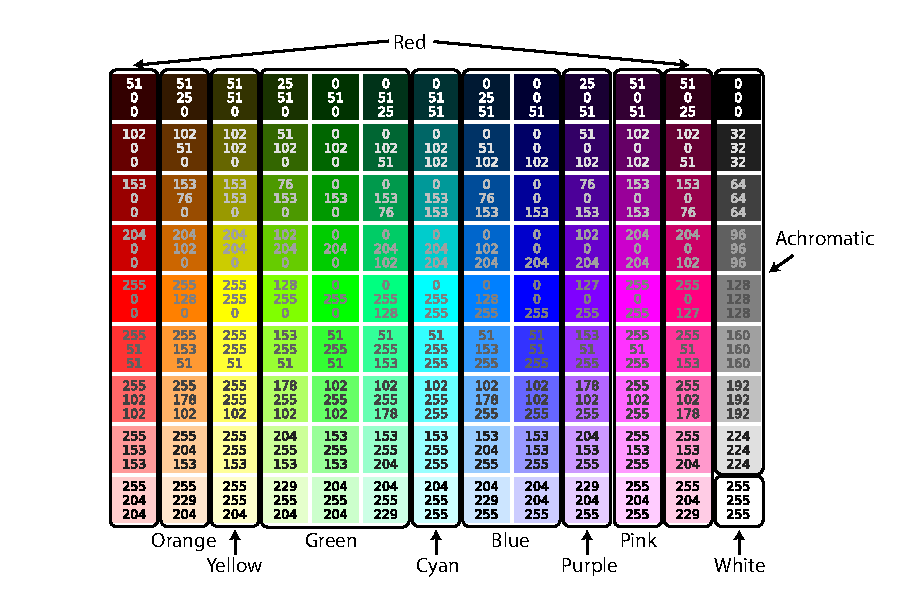
\includegraphics[width=0.5\textwidth]{figures/Col_tab.pdf}
	\caption{Set of 117 colours aggregated in 10 groups. For each colour, the three values represent the RGB components. \label{fig:colour_set}}
\end{figure}

Then, for each pixel \(\vec{s}\), the less dissimilar \(c_l\) is considered as
the colour of the pixel:
\begin{equation*}
c(\vec{s}_{ij}) := \operatornamewithlimits{argmin}_{l \in [1,L]} \| s_{ij} - c_{l} \|^{2}
\end{equation*}

{\color{red}[Other distances tested, such the one from Androutsos 1999 et un autre plus récent et mieux, add ref in 4.1 for fig. 3]}

Finally, according to the Figure~\ref{fig:colour_set}, the 117 colours are grouped into $G = 10$
main colours ($g = 1, \dots, G$), \textit{i.e.} red, orange, yellow, green, cyan, blue, purple, pink,
white and achromatic. Therefore, each pixel belongs to one of these
$G$ groups and the name of the colour of each pixel is defined as {\color{red}$C(\vec{s}_{ij}) = g \quad \textrm{if} \quad c(\vec{s}_{ij}) \in g$}. \footnote{Here and in the sequel, $\mathds{1}(A)$ denotes the \textit{indicator function} of event $A$, taking on the value 1 if $A$ is true, and 0 otherwise.}

For each drawing $k$, this permits us to obtain one
boolean matrix per colour $g$:
\begin{equation}
B^{g} = (b_{ij}^{g}) \quad \textrm{with} \quad b_{ij}^{g} =  \mathds{1}(C(\vec{s}_{ij}) = g)
\end{equation}

Thus, the \textit{count of pixels}  (\textit{i.e.} the number of pixels) of each main colour $g$ for one drawing is defined as:
\begin{equation}
	n^{g} = \sum_{ij}b_{ij}^{g}
\end{equation}


It is important to note that the set of $L=117$ colours is based on a typical RGB colour chart~\footnote{such as the one available on: \url{https://www.rapidtables.com/web/color/RGB_Color.html}}, bur another one could be used. Regarding the set of main colours $G$, it is a result of discussions in the project team, as explained in section~\ref{sec:set_col_definition}. Black and grey were grouped into achromatic, since it is complicate to differentiate these two colours (or which pencil was used by the children), for a computer, as well as for an human. Moreover, this distinction is not necessary to study a child's colour choice. Furthermore, brown is not included in the colour list, since it is difficult to define according to the method described above and the colour space chosen. However, it would be possible to group some of the 117 colours into a new group ``brown''. Similarly, it is possible to create a complete different set of main colours. For instance, blue and cyan could be grouped.
{\color{red} ** PYB **, QUELQUE CHOSE A AJOUTER?}

Therefore, we are able to attribute one colour per pixel and thus, extract the proportion of
each colour used in each drawing (see section~\ref{sec:results_identification}), in order to answer the first type of psychological research questions mentioned in section~\ref{sec:introduction}. 
Regarding the second type of questions, the proposed methods are explained in the next section.



{\color{red}[MET-ON LE CODE SUR GITHUB??? ET ENSUITE UN LIEN?]}


\subsection{Colour diversity [ARIS]}
\label{sec:diversity}


There are a number of ways of quantifying the diversity associated with a discrete distribution, such as the distribution of colours in a drawing obtained with the identification method described in section~\ref{sec:identification} above. All diversity measures are, to a certain extent, dependent on the size of the sample from which the considered distribution has been obtained \cite[see e.g.][]{TweedieBaayen1998}, however the impact of this dependence is lessened in our case by the (partial) normalisation of drawing size (see section~\ref{sec:preprocessing} above). In the present study, we experiment with two diversity measures, namely the {\em variety} or number of distinct colours in a drawing, and the {\em Shannon entropy} of the colour distribution.

In the case of variety, an additional preprocessing step is performed: in order to reduce the amount of noise--anomalous pixels resulting from the digitisation process--a median filter of \(3 \times 3\) pixels is applied to each boolean colour matrix $B^{g}$. The filtered matrix, $\tilde{B}^{g}$, is then used to compute new counts $\tilde{n}^{g} = \sum_{ij}\tilde{b}_{ij}^{g}$, which in turn make it possible to calculate the colour variety as:
\begin{equation}
	V = \sum_{g}\mathds{1}(\tilde{n}^{g} > 0)
\end{equation}

Following \citet{Shannon1948}, the colour entropy is defined as:
\begin{equation}
	H = -\sum_{g} f^{g}\mbox{ log }f^{g}
\end{equation}
where $f^{g}:= n^{g}/\sum_{k}n^{k}$ stands for the (unfiltered) colour relative frequency. $H$ varies between 0 and log $G$: $H=0$ corresponds to a deterministic configuration where a single colour occurs with relative frequency $f^{g} = 1$, while the maximum $H=\mbox{log }G$ is reached when the colour distribution is uniform ($\forall g: f^{g} = 1/G$).



\section{Results [RAPHAEL]}
Here, we first show an explicit sample of the results obtained from the method Identification of colours (see section \ref{sec:identification}) applied on all drawings. 
We then extend the presentation of these results using the method of Colour diversity retrieval (see section \ref{sec:diversity}) crossed with the results of a deeper measure of variety commonly used in Computer Vision. 
The results of the Colours space definition experiment depicted in section \ref{sec:set_col_definition} are presented in order to asses the automatic method of variety estimation in face of human perceived variety.

\subsection{Colour identification}
\label{sec:results_identification}
The colour identification step yields the boolean $B^g$ matrix per colour $g$ for each $k$ drawing from where masked-image can be reconstructed to reveal the colour configuration of the original drawing as illustrated on Figures~\ref{fig:example1}~and ~\ref{fig:example2}.

\begin{figure}[!h]
	\centering
	\raisebox{0.45cm}{\includegraphics[width=0.32\linewidth]{figures/ru08_bo_f_pb_07_05_ali-r.jpg}}
	\includegraphics[width=0.62\linewidth]{figures/ru08_bo_f_pb_07_05_ali-rno_filter_mask.pdf}\hfil
	\caption{Good illustration of the colour identifications: Russian drawing.}
	\label{fig:example1}
\end{figure}

\begin{figure}[h!]
	\centering
	\includegraphics[width=0.32\linewidth]{figures/ch15_fr_m_rrs_08_08_fim-r.jpg}
	\includegraphics[width=0.62\linewidth]{figures/ch15_fr_m_rrs_08_08_fim-rno_filter_mask.pdf}
	\caption{Less good illustration of the colour identifications: Swiss drawing.}
	\label{fig:example2}
\end{figure}

\

The first figure illustrates a good extraction of the main colours whereas the second illustrates a less good colour extractions because of the similar computed distances between $\vec{s}$  pixel and the two or more $G$ main colours e.g. $g = \mbox{Green}$ and $g = \mbox{Achromatic}$. 
Also, the lack of the main colour  Brown in the defined set of colours produces errors during the colours identification process as well as a over attribution of the pixels to the Green when yellow and grey overlap into the drawing. 
{\color{red}[CC:  Parler des bons resultats v.s. mauvais resultats avec examples (qui sont encore \`a choisir)]}.

\

From there, we compute the proportion of coloured pixels per $g$ colour, where $g \in G \not\ni g = white$, to reveal the weighted frequency of main colours (see Figure \ref{fig:propcolours}). 
For this dataset, the results obtained allows to said that the Achromatic is the most identified followed by the Blue and the Yellow whereas the Pink and the Purple are clearly less present (they represent $70.3\%$ against $0.9\%$). The Orange, Red, green and Cyan seem to be moderately present ($27.8\%$). 
{\color{red} ** P.-Y.B. **}

\ 

{\small \color{teal}[IDEE: Cross validation en prennant al\' eatoirement quelques pixels par dessin et les attribuer manuelle \`a une couleurs principales ou avoir un toy example avec un dessin o\`u l'on "connait" les couleurs.]}

\begin{figure}[h!]
	\centering
	\includegraphics[width=\linewidth]{figures/colors-barplot.png}
	\caption{Proportion of coloured pixels per $g$ colour, where $g \in G \not\ni g = white$.}
	\label{fig:propcolours}
\end{figure}


\subsection{Colour diversity}
\label{sec:results_diversity}
However we are able to identified automatically colours with a specific chosen set of colours, the colour variety of the drawing still not considered. 

\subsubsection{Entropy and variety}
Based on the colours identifications results, we then compute the relative entropy {\color{red}[Ajouter ref. \'equation quand disponible]} as well as the variety in order to reveal, first, the proportional colour variety of the dataset and, secondly, to compare it with the absolute variety of the dataset, number of non-empty main colours $g$, see Figure~\ref{fig:boxplotvariety}.
Globally, the medians of the boxes indicate an linear  relationship between the entropy and the variety, whereas the absolute frequency of drawings per number of colours identified, the variety, has an normal distribution.

\begin{figure}[h!]
	\centering
	\includegraphics[width=\linewidth]{figures/colors-boxplot.png}
	\caption{Entropy $H(f)$ box plot for the $N$ drawings per the numbers of colours identified, namely the variety $m$.}
	\label{fig:boxplotvariety}
\end{figure}

\begin{figure}[h!]
	\centering
	\includegraphics[width=0.8\linewidth]{figures/colors-grille.png}
	\caption{Sample of drawings, selected per quartiles, and ordered by entropy (column) and variety (row). {\color{red}[AJOUTER ENCORE LE AXES]}}
	\label{fig:grille}
\end{figure}

In more details, we observe on Figure \ref{fig:grille} that the entropy value attached to each drawing indicates a degree of completeness: the higher the entropy value is, more the colours are covering the page revealing more complex drawings whereas the lower values depicts lower coloured and complex drawings where $H(f) \rightarrow 0$ reveals whiter pages.
Also, combined with the variety, we observe that measure allows a gradual distinction between white drawing background with a single object to drawing with more contextualized (mutli-)object(s).
{\color{red} ** P.-Y.B. **}


Based on the chosen colour sets, the entropy measure is sensitive to the errors during the pixel colour attributions (e.g. similar distances, no Brown, etc.). 
Then, we compare it with a common approach of Computer Vision which consists to measure the entropy on the greyscale levels histogram of the drawing. 
The scatter plot, figure~\ref{fig:entropies}, depicts the significant Pearson correlation ($r=0.8866$, $p=0.000$) between these two entropy values {\color{red}[Reprendre quelques parties de 3.5 et citer \citet{wu2013}]}. 

{\small \color{teal}[IDEE: Est-ce que les extr\`emes ne permettraient pas d'en dire plus? A creuser.]}

\begin{figure}[h!]
	\centering
	\includegraphics[width=\linewidth]{figures/colors-greysacale-entropies.png}
	\caption{Scatter plot of the entropies on the greyscale levels histogram with the main colours entropies.}
	\label{fig:entropies}
\end{figure}

\subsubsection{Variety concordance}

For each $i$ drawing in a sample of $\tilde{N} = 10$ drawings, we evaluate the concordance of the variety computed automatically $v^c_i = {1, \dots, G}$, by the algorithm of section \ref{sec:identification}, and the human perceived variety $v^h_i = {1, \dots, +\infty}$. 

\

First, we observe on Figure~\ref{fig:compnbcolourssd} that the numbers of colours identified automatically is different to the humans in a range of two colours in average. 
These results are quite impressive in face of the number of factors considered during both estimations of variety; on one hand the errors of the automatic attributions observed previously and, on the other hand, the human perception bias. 
The Figure \ref{fig:compnbcoloursscatter} confirms this trend with a linear relationship.

\begin{figure}[h!]
	\centering
	\includegraphics[width=\linewidth]{figures/comp_nb_colours_sd.png}
	\caption{Drawings in function of the means numbers of colours estimated by the algorithm and human.}
	\label{fig:compnbcolourssd}
\end{figure}

\begin{figure}[h!]
	\centering
	\includegraphics[width=\linewidth]{figures/comp_nb_colours_scatter.png}
	\caption{Scatter plot of the variety observed by human in function of the automatic estimation of the variety.}
	\label{fig:compnbcoloursscatter}
\end{figure}

\

The Figure~\ref{fig:blandandaltman} shows the range of the disagreement using the \textit{Bland and Altman graphic} \cite{bland1986}.
The differences between the varieties of each $i$ drawing,  $d_i = v^c_i - v^h_i$, are represented in function of their means $\overline{d}_i = v^c_i + v^h_i/2$. 
The range of disagreement $d_i$ is then analysed in function of the mean $\overline{d}_i$. More $d_i$ is distant of  $0$, respectively close, $d_i \rightarrow 0$ , more the disagreement is higher, respectively concordant,  whereas $\overline{d} = 1/N\sum_{i}^{\tilde{N}}d_i = 0$ depicts a perfect concordance between these two varieties. 

\

Although there is no significant disagreement under the normal distribution hypothesis, the low size $\tilde{N}$ of the sample is not representative and show already a mean disagreement $\overline{d}=?$ {\color{red}[AJOUTER LA VALEUR DE D\'ESACCORD]}.


\begin{figure}[h!]
	\centering
	\includegraphics[width=\linewidth]{figures/comp_nb_colours_agreement.png}
	\caption{Range of disagreement of variety estimations using Bland et Altman  Graphic.}
	\label{fig:blandandaltman}
\end{figure}



\section{Conclusion}

{\color{red}[TO UPDATE AT THE END] }
{\color{gray} As a next step, since humans are more sensitive to colour patches than

to isolated pixels, a filter should be applied at the beginning of the
process, such as the Mumford-Shah Regulariser proposed by
\citet{erdem2009}. Indeed, when children (or adults) fill in an area of
the sheet with colour, the application is not regular and consequently
not all pixels of the zone are coloured. Thus, in order to avoid
underestimating the proportion of one particular colour, standardizing
colours by zone could help work around the possible issue.}

These methods are
applicable to other data and research, e.g.~studying the main colours
used by a painter according to various periods of his/her life.

Moreover, as explained in section..., it is possible to define a different set of colours and/or to start with more or less than 117 colours.

Later: define and detect brown.

\bibliography{bibliography}
\bibliographystyle{acl_natbib}

\end{document}
